\chapter{Confronto}
\section{Il database}
Il database di entrambi gli strumenti è un aspetto cruciale per la qualità e l'accuratezza delle analisi di vulnerabilità. Trivy e Snyk utilizzano database di vulnerabilità differenti, che influenzano la loro capacità di identificare e classificare le vulnerabilità. Trivy si basa su VulnDB, un database di vulnerabilità curato da Risk Based Security, che offre una copertura dettagliata e aggiornata delle vulnerabilità di sicurezza. Snyk, d'altro canto, utilizza un database di vulnerabilità proprietario, che combina dati provenienti da diverse fonti, inclusi i database NVD, NPM, RubyGems e altri. Questo approccio permette a Snyk di offrire una copertura più ampia e dettagliata delle vulnerabilità, ma può comportare un rischio di falsi positivi e falsi negativi, a causa della complessità e della varietà dei dati raccolti. Trivy, invece, offre una copertura più limitata, ma più accurata e affidabile, grazie alla cura e all'attenzione dedicata da Risk Based Security alla qualità dei dati e alla loro classificazione.
In questa parte di testing, si è voluto valutare la capacità di Trivy e Snyk di identificare e classificare le vulnerabilità in base al database utilizzato. Per fare ciò, si è utilizzato un campione di immagini di container e repository Git, contenenti vulnerabilità note e ben documentate, e si è confrontato il risultato delle scansioni di Trivy e Snyk con le informazioni disponibili nei database VulnDB e Snyk. I risultati di questo test sono stati valutati in base alla precisione, alla completezza e alla tempestività delle informazioni fornite da Trivy e Snyk, e alla loro capacità di identificare e classificare le vulnerabilità in base al database utilizzato.
L'aggiornamento dei database avviene per ogni tool in modo differente. Trivy, infatti, controlla la presenza di aggiornamenti del database ad ogni esecuzione, e scarica automaticamente la versione più recente. Snyk, invece, offre la possibilità di aggiornare manualmente il database, ma non è possibile controllare la presenza di aggiornamenti in modo automatico.

Le immagini Docker sottoposte a scansione sono state selezionate in base alla loro popolarità e alla loro rilevanza nel panorama delle applicazioni e dei servizi cloud. In particolare, si è scelto di testare le seguenti immagini:
\begin{itemize}
   \item \textbf{nginx:latest}: una delle immagini di container più popolari e utilizzate, che offre un server web leggero e performante basato su Nginx.
   \item \textbf{mongo:latest}: una delle immagini di container più popolari e utilizzate, che offre un database NoSQL flessibile e scalabile basato su MongoDB.
   \item \textbf{wordpress:latest}: una delle immagini di container più popolari e utilizzate, che offre una piattaforma di blogging e CMS basata su WordPress.
   \item \textbf{alpine:latest}: una delle immagini di container più leggere e minimali, basata su Alpine Linux, che offre un ambiente di esecuzione ideale per applicazioni e servizi cloud.
   \item \textbf{centos:latest}: una delle immagini di container più stabili e affidabili, basata su CentOS, che offre un ambiente di esecuzione robusto e ben supportato per applicazioni e servizi cloud.
\end{itemize}
I risultati rilevati da entrambi i tool sono riportati nella tabella seguente:
% Tabella da aggiungere successivamente
\section{Utilizzo in pipeline CI/CD}

\section{Differenze di funzionalità}
Durante il testing, sono state rilevate le seguenti funzionalità uniche per ciascuno strumento:
\subsection{Trivy: scansione di cluster Kubernetes}
Trivy offre la possibilità di eseguire la scansione di un intero cluster Kubernetes, identificando e classificando le vulnerabilità presenti nei pod, nei deployment e nei servizi. Questa funzionalità è particolarmente utile per i team di sicurezza e per gli amministratori di sistema, che possono utilizzare Trivy per identificare e mitigare le vulnerabilità in modo proattivo, prima che possano essere sfruttate da attaccanti. Durante il testing, si è verificato che Trivy è in grado di eseguire la scansione di un cluster Kubernetes in modo rapido ed efficiente, fornendo un report dettagliato delle vulnerabilità rilevate e delle azioni consigliate per mitigarle.
\subsection{Trivy: Scansione delle Configurazioni Infrastructure as Code (IaC)}
Trivy offre la possibilità di eseguire la scansione delle configurazioni Infrastructure as Code (IaC), identificando e classificando le vulnerabilità presenti nei file di configurazione di Terraform, CloudFormation e altri strumenti di automazione dell'infrastruttura. Questa funzionalità è particolarmente utile per i team di sviluppo e per gli amministratori di sistema, che possono utilizzare Trivy per identificare e mitigare le vulnerabilità nelle configurazioni IaC, prima che possano essere sfruttate da attaccanti. Durante il testing, si è verificato che Trivy è in grado di eseguire la scansione delle configurazioni IaC in modo rapido ed efficiente, fornendo un report dettagliato delle vulnerabilità rilevate e delle azioni consigliate per mitigarle.
\subsection{Trivy: }

\subsection{Snyk: Monitoraggio Continuo}
Snyk offre un monitoraggio continuo delle applicazioni e delle dipendenze, inviando notifiche in tempo reale in caso di nuove vulnerabilità che influenzano il codice già in uso. Questo assicura che i team possano reagire rapidamente a nuove minacce. Durante il testing, è stato possibile osservare il funzionamento di questa funzione, avendo ricevuto e-mail contenenti nuove vulnerabilità pubblicate solamente giorni prima, come riportato in figura \ref{fig:snyk_email}.

\begin{figure}[H]
   \centering
   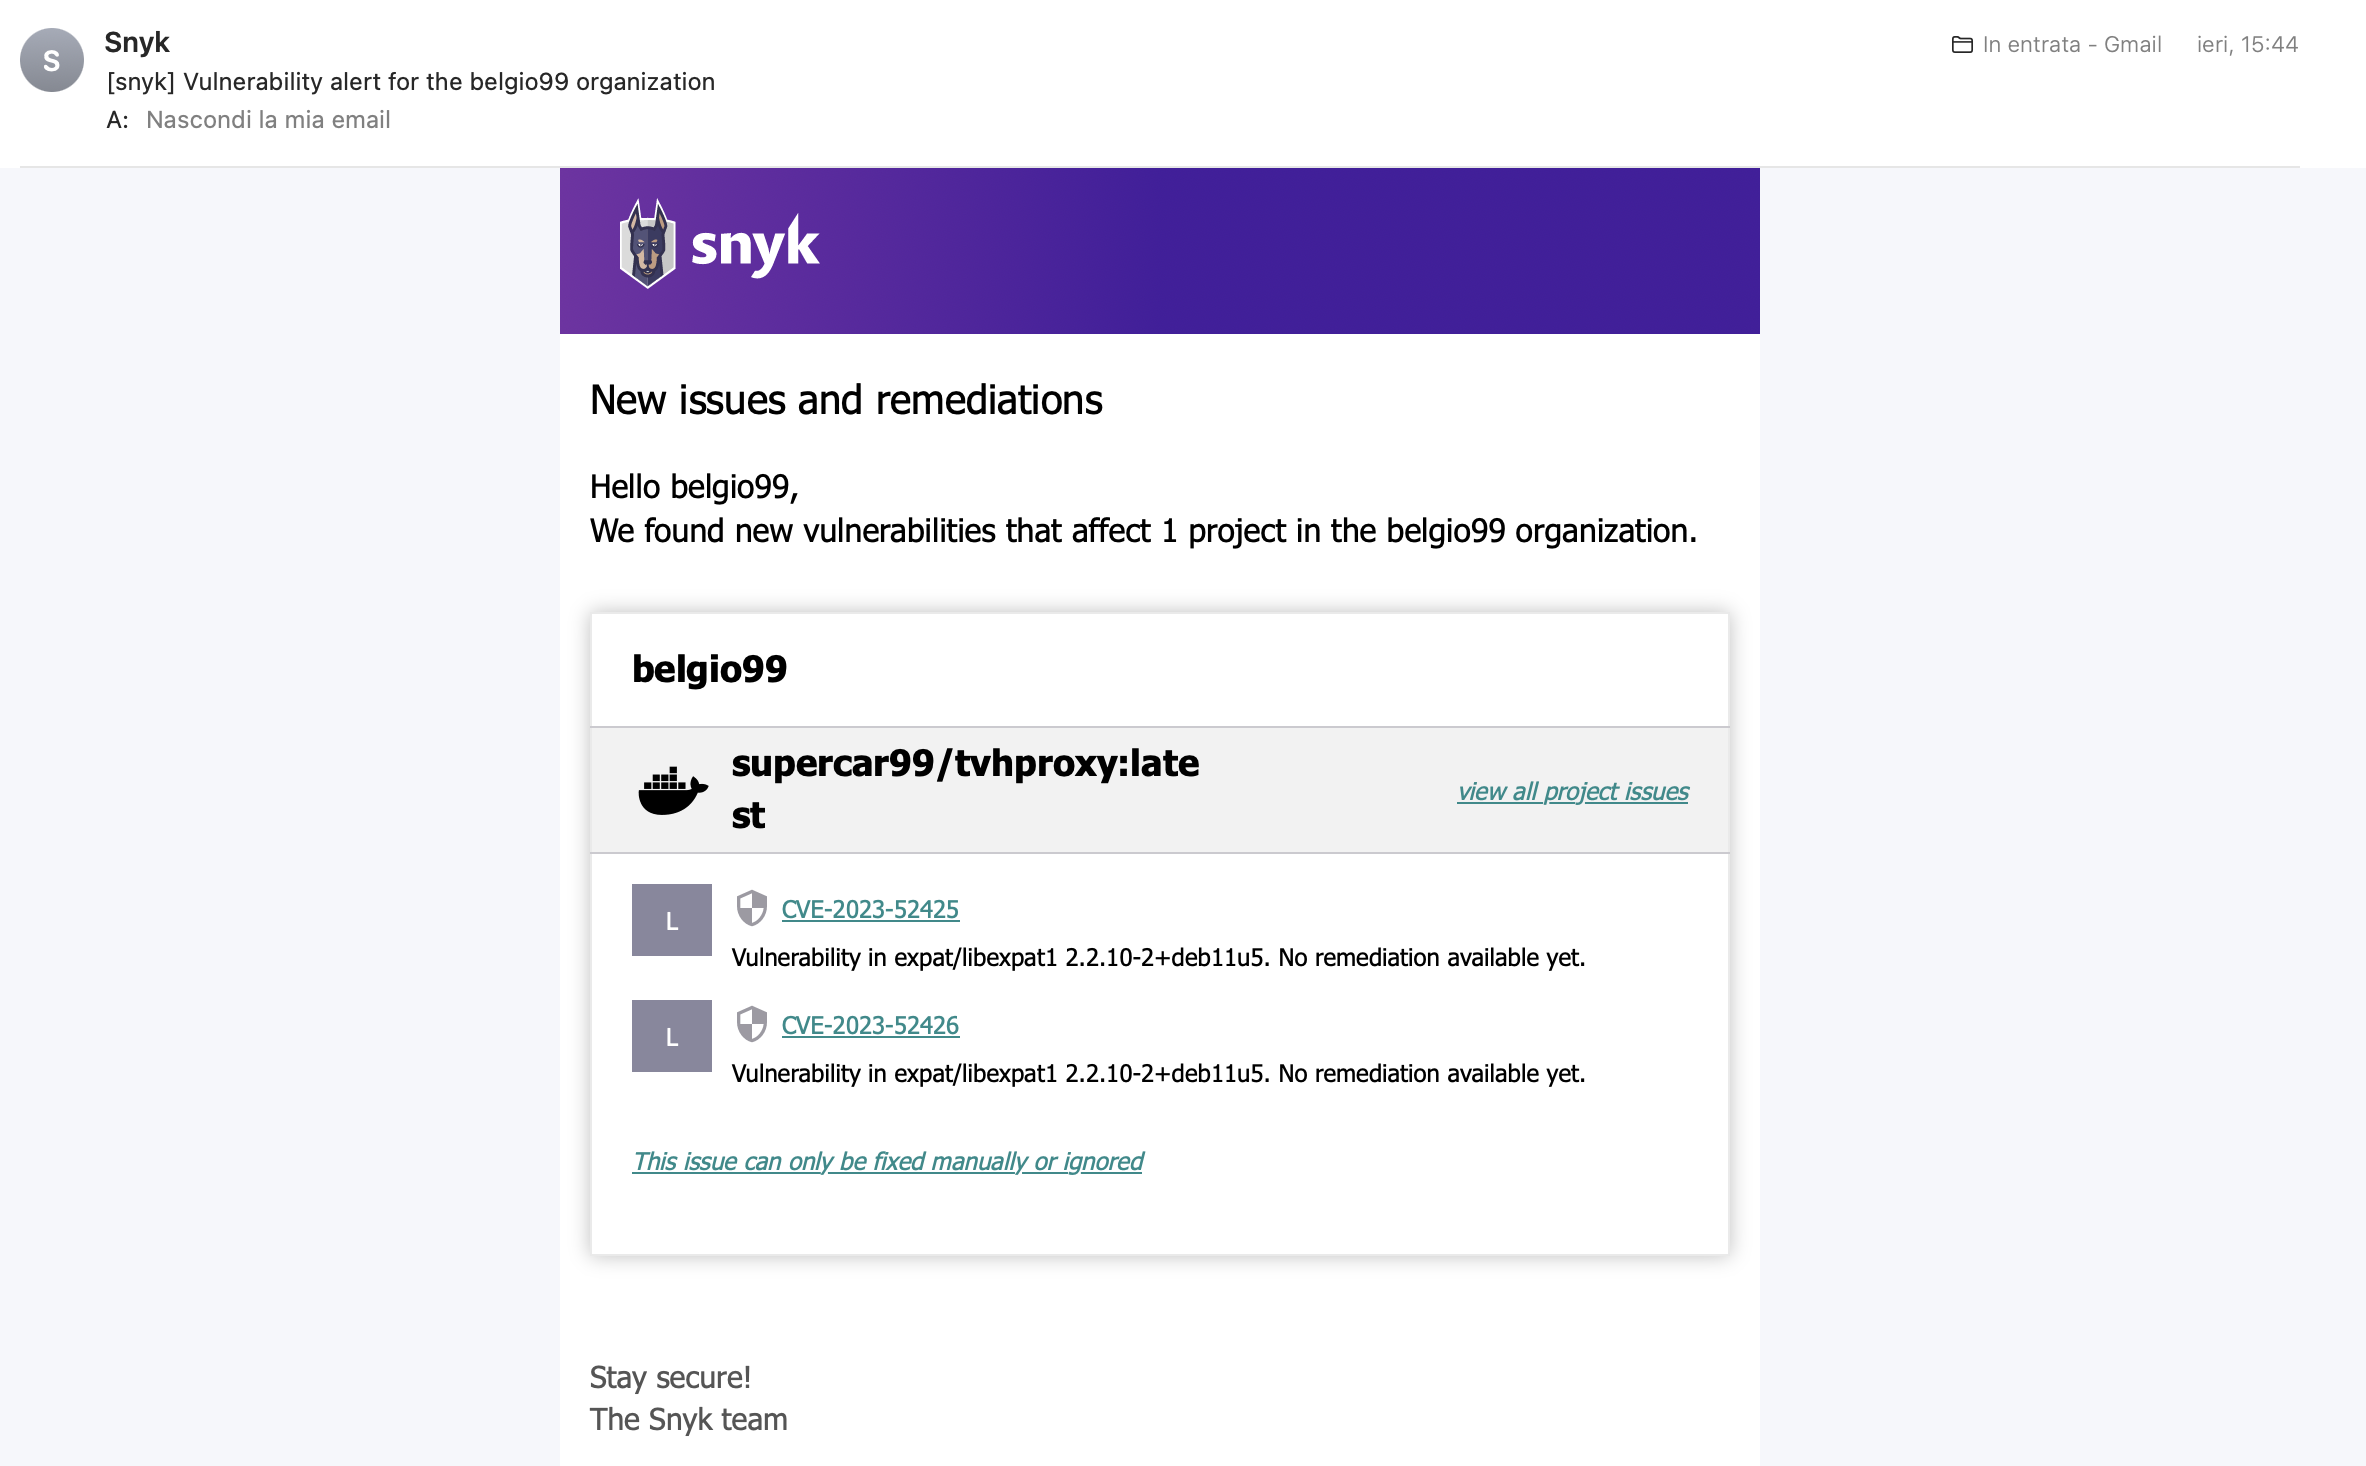
\includegraphics[width=0.8\textwidth]{immagini/capitolo2/snyk_email.png}
   \caption{E-mail ricevuta da Snyk contenente notifica di rilevazione di nuove vulnerabilità}
   \label{fig:snyk_email}
\end{figure}

Dopo la ricezione della e-mail, è stata subito eseguita una scansione con Trivy, che ha confermato la presenza delle vulnerabilità segnalate da Snyk. Questo conferma che entrambi i database utilizzati da Trivy e Snyk sono aggiornati tempestivamente.